\subsubsection{D\'efinition des graphes Iourtes}

\begin{figure}[htb!] 
\centering
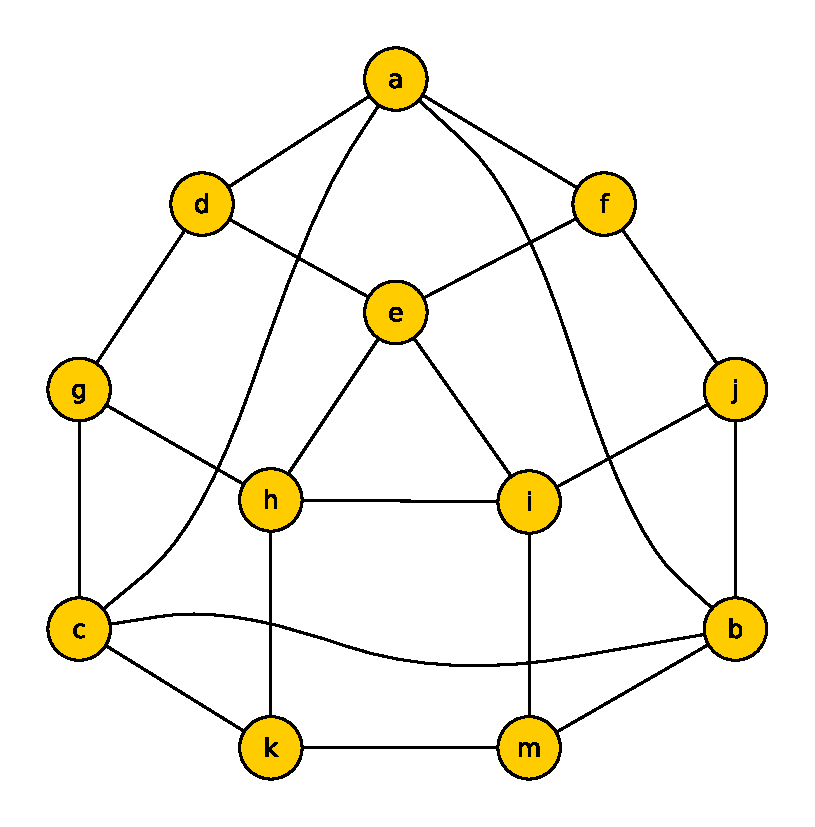
\includegraphics[scale=0.50]{grapheIourteG0.eps}
\caption{Graphe $G_0 $}
\label{grapheIourteG0} 
\end{figure}

\begin{definition}
Le graphe $G_0 = (V, E)$ est un graphe dont
\begin{itemize}
	\item l'ensemble $V$ contient $12$ sommets et l'ensemble $E$ a $21$ ar\^etes ($|V| = 12, |E| = 21)$.
	\item soit $N(v)$ l'ensemble des sommets adjacents \`a $v$. 
		les sommets $N(v)$ ne forment pas de cliques. \newline
		$\forall v \in V, \forall u, u' \in N(v),  (u, v) \in E \hspace{1 em} et  \hspace{1 em} (u, u') \notin E $
	\item $G_0$ est {\em 4-r\'egulier}.
\end{itemize}
\end{definition}
%La figure \ref{grapheIourteG0} d\'esigne le graphe $G_0$.
%En modifiant trois ar\^etes de $G_0$ en une chaine de longueur $2$, j'obtiens le graphe  $G_0^1$ de $15$ sommets et $27$ ar\^etes.
%De m\^eme, le graphe  $G_0^2$, de $18$ sommets et $30$ ar\^etes, se determine en modifiant encore trois ar\^etes de $G_0^1$  en une chaine de longueur $2$.
%En appliquant recursivement $k$ modifications sur le graphe $G_0$, nous avons le graphe $G_0^k$.
%Nous designons par $k$, la profondeur du graphe $G_0$.

\begin{definition}
Un graphe Iourte $G_0^k$ est une paire $(G_0, k)$ dans laquelle nous  augmentons les ar\^etes de $G_0^{k-1}$ de $3$ en remplacant  $3$ ar\^etes de $G_0^{k-1}$ en une chaine de longueur $2$.
\end{definition}
Nous d\'esignons par $k$, la profondeur du graphe $G_0$.
En substituant  les trois ar\^etes [a,c],[b,c],[c,a] de $G_0$ en des chaines de longueur $2$, nous obtenons le graphe  $G_0^1$ de $15$ sommets et $27$ ar\^etes. 
Nous cr\'eons $3$ sommets a',b',c' et leurs voisins sont respectivement $a$ et $b$, $b$ et $c$, $c$ et $a$ (voir figure \ref{grapheIourteProfondeur2}).
\begin{figure}[htb!] 
\centering
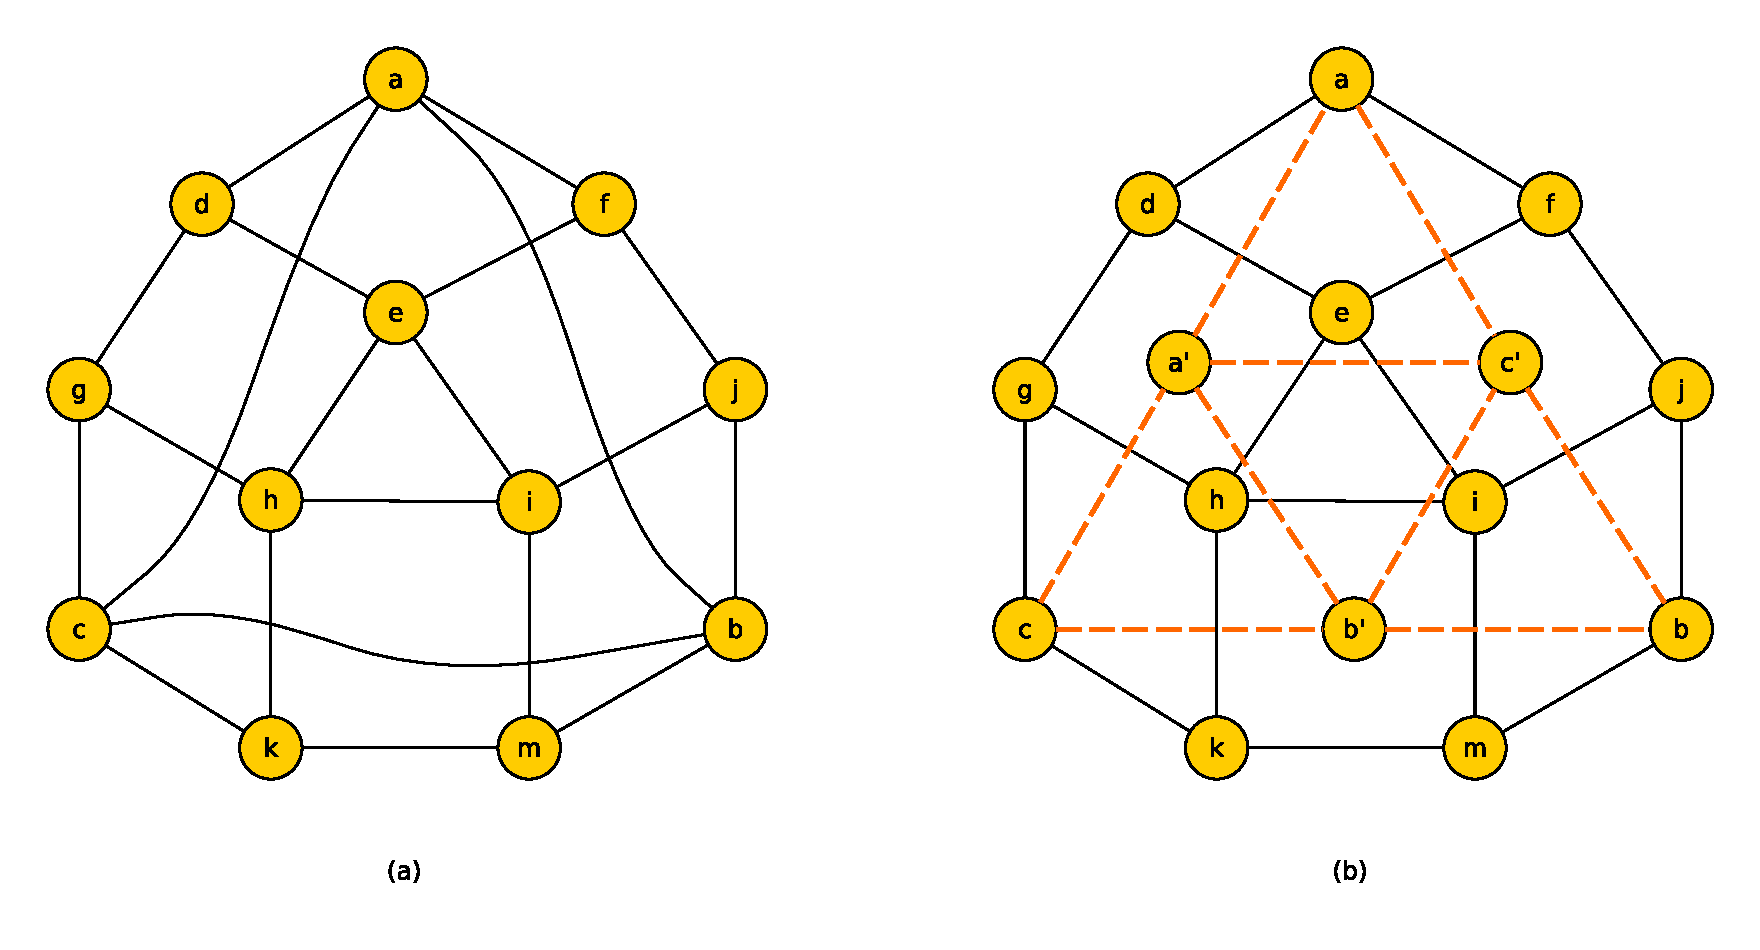
\includegraphics[scale=0.50]{grapheIourteG0Profondeur1.eps}
\caption{ (a): Graphe $G_0$. (b): Graphe $G_0^1 $ : ajout de sommets a', b' et c'  et des ar\^etes en pointill\'ees de couleur rouge.}
\label{grapheIourteG0Profondeur1} 
\end{figure}
\newline
Ainsi, pour obtenir $G_0^2$, nous modifions les ar\^etes $[a',b']$,$[b',c']$ et $[a',c']$. On en d\'eduit que:

\begin{theorem}
Le graphe $G_0^k$ est un graphe iourte de $3k+12$ sommets et $6k + 21$ ar\^etes
\end{theorem} 

\begin{proof}
Nous distinguons trois sommets $A$, $B$, $C$ dans $G_0$. 
\`A partir de $G_0$, nous obtenons $G_0^1$ en ajoutant $3$ sommets par les modifications  suivantes.
Nous remplacons chaque ar\^ete $[A,B]$, $[B,C]$,  $[A,C]$  par une chaine de longueur $2$. 
Les sommets ainsi cr\'ees deviennent les nouveaux sommets   $A$, $B$, $C$ qui forment un cycle de longueur $3$.
Ainsi le voisinage de ces $3$ sommets  ne peut pas \^etre couvert par une ou deux cliques.
En rep\'etant $k$ fois cette modification, nous obtenons le graphe $G_0^k$ de $3k+12$ sommets et $6k+21$ ar\^etes.
\end{proof}

\subsubsection{Correction du graphe Iourte  $G_0^k$}
Nous appliquons maintenant le couple d'algorithmes aux graphes Iourtes $G_0^k$.
La figure \ref{grapheIourteG01eExecution} d\'ecrit un line-graphe $L(G_0)$ couvrant $G_0$ en lui ajoutant $6$ ar\^etes (en pointill\'ees).
La s\'election des sommets \`a corriger est $h, e, f, g, b, j, m$. 
Les sommets ne figurent pas dans cette s\'election parce qu'ils n'ajoutent ou suppriment aucunes ar\^etes et ne modifient pas les cliques d\'ej\`a trouv\'ees.
Ces $6$ ar\^etes d\'esignent la plus petite modification possible de $G_0$ en termes de co\^ut d'ajout et suppression.
Par cons\'equent $DL(G_0) = 6$. 
\begin{conjecture}
\label{conjectureDLIourte}
La distance line de $G_0^k$ v\'erifie $DL(G_0^k) \le 3k+6$.
\end{conjecture}
\begin{figure}[htb!] 
\centering
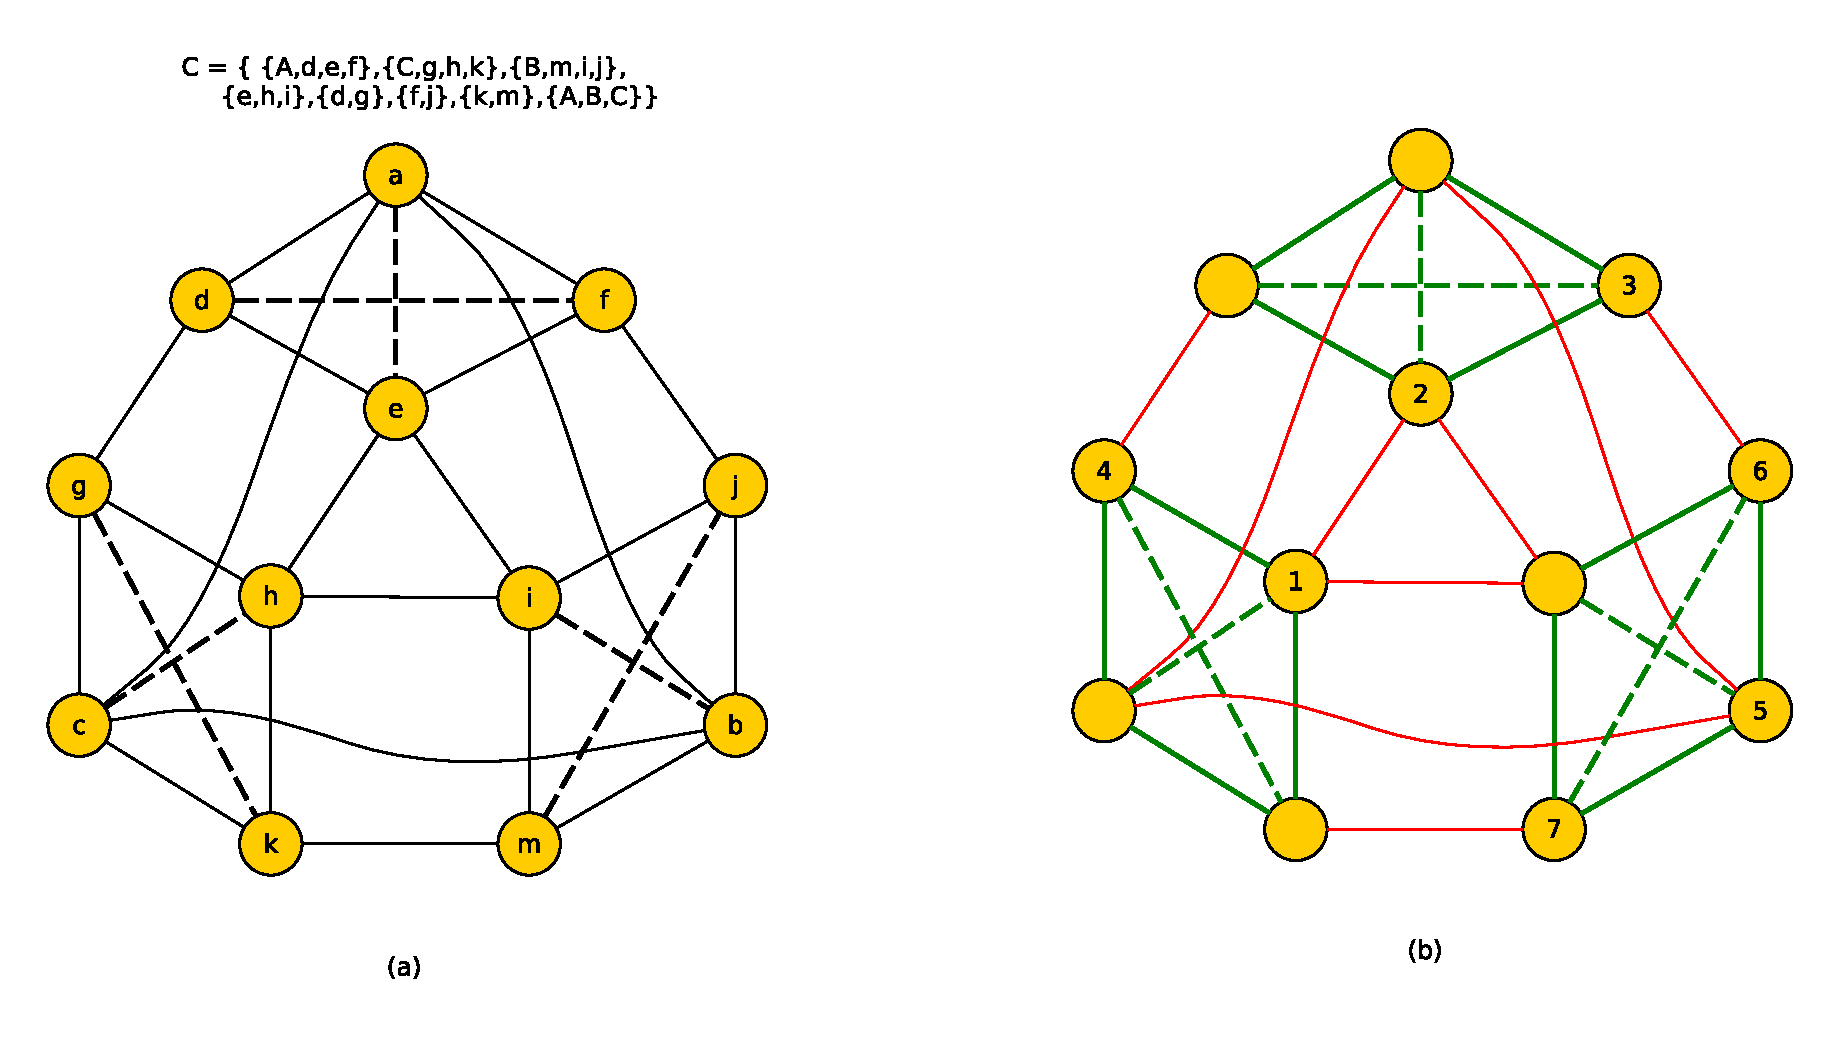
\includegraphics[scale=0.50]{grapheIourteG01eExecution.eps}
\caption{Une correction du graphe $G_0$ : $DL(G_0) = 6$ }
\label{grapheIourteG01eExecution} 
\end{figure}
Le line-graphe  $L(G_0^k)$ couvrant $G_0^k$ ayant une distance de Hamming de $3k+6$ s'obtient \`a partir de  $L(G_0^{k-1})$ en supprimant une ar\^ete parmi deux dans un cycle de taille $6$. Ce cycle est form\'e par les anciens sommets $A$, $B$, $C$ (de $G_0^{k-1}$) et les nouveaux sommets $A$, $B$, $C$ de $G_0^k$, soit une suppression de $3$.
Chaque ar\^ete non supprim\'ee dans ce cycle forme une clique de taille $2$ et  le nouveau cycle de taille $3$ entre les sommets $A$, $B$, $C$ forme une nouvelle clique (en rempla\c cant la pr\'ec\'edente clique de $L(G_0^{k-1})$).